\subsection{Fully-Leptonic} \label{sec:FullyLeptonicEventSelections}


For events to fall into the FL analysis category, they must contain exactly two oppositely charged leptons ($e^{+}e^{-}$, $\mu^{+}\mu^{-}$, $e^{\pm}\mu^{\mp}$).
The leading \pt lepton is required to have \pt $>$ 20 GeV, the subleading lepton is required to have \pt $> 10GeV$, and a distance parameter between the two leading \pt leptons $>$ 0.4 is required.
Events are rejected from this category if the event contains a third lepton with \pt $> 10$ GeV in order to avoid saving events with three high energy leptons, as only two 
are expected from this process. In order to identify events with missing transverse momentum due to the two neutrinos from the 
leptonically decaying W-bosons, events are required to have $p_T^{miss} > 20$ GeV. Furthermore, the diphoton candidate in this final state is required to have \pt $> 91$ GeV, 
and the invariant mass between each electron candidate and photon candidate is required to be at least 5 GeV different from the invariant Z boson mass to avoid saving Z$\rightarrow\ell\ell$ events. The invariant mass 
from the two leading leptons is required to be $<$ 80 GeV or $>$ 100 GeV in order to suppress VH(H$\rightarrow\gamma\gamma$) events, as shown in Fig \ref{fig:FL_support}. In addition, events containing at least one jet 
with a b-tagging score greater than a medium working point are removed. The reason a b-veto is applied in this final state and not for the SL and FH final states is because this final state applies 
a cut-based selection, and therefore we choose to apply a b-veto as part of the final selections. 

% The cut based Fully-leptonic analysis is performed for both the SM and EFT interpretations. In this channel, events are required to contain a diphoton candidate passing preselection, and at least two oppositely charged leptons ($e^+\ e^-$,$\mu^+\ \mu^-$,$e^{\pm}\ \mu^{\mp}$). % by definition, all events contain MET, so no need to specify here.
% The diphoton candidate and its leading and subleading photons must pass the common event selections described in Section ~\ref{sec:commomSel}, % there is no common MET selection.
% and leptons must pass the electron and muon object selections described in Tables \ref{tab:ElectronSelections} and \ref{tab:MuonSelections} to suppress background, but preserve enough statistics to constrain background models.
% Events are required to satisfy the selections listed in Table \ref{tab:FLSelections}.

% For the Fully-Leptonic final state category, the medium bveto working point is applied as only about 5\% of signal is rejected, while about 85\% of ttHJetToGG background is rejected.
% An event is vetoed if it contains at least one jet with a DeepFlavour bscore greater than the medium working point. The reason a b-veto is applied in this final state and not for the semi-leptonic 
% and fully-hadronic final states is because this final state applies a cut-based selection, and therefore we choose to apply a b-veto as part of the final selections. 

% \begin{table}[!htbp]
%     \begin{center}
%         \begin{tabular}{c|c}
%         Variable & Selection \\ \hline
%         $\Delta{R(l,l)}$ & $> 0.4$ \\
%         Number of leptons & $= 2$ \\
%         The \pt of leading lepton & $> 20GeV $\\
%         The \pt of subleading lepton & $> 10GeV$ \\
%         $E_T^{miss}$ & $> 20GeV$ \\
%         $p_T^{\gamma\gamma} $ & $> 91 GeV$ \\
%         $| m_{e\gamma} - m_Z |$ & $>5 GeV$ \\
%         $m_{ll}$ & $<80 GeV\ or >100 GeV $
%         \end{tabular}
%     \end{center}
%     \caption{
%       Requirements of Fully-Leptonic Channel
%     }
%     \label{tab:FLSelections}
% \end{table}

% Where Table \ref{tab:FLSelections} variables have the following definitions:
% \begin{itemize}
%   \item $\Delta{R(l,l)}$ is the $\Delta{R}$ between two leptons
%   \item $m_{ll}$ is the mass of dilepton system
% \end{itemize}

The $p_T^{\gamma\gamma}$ selection was chosen to optimize $\frac{S}{\sqrt{B}}$ while also preserving enough events for a meaningful background fit.
The significance plot is shown in Fig.~\ref{fig:FL_support} (a).
Working points were identified from this plot for which limits are computed, and a study is performed to determine if the data-driven background model fit introduces a bias in the signal region.
The results from these checks are shown in Table \ref{tab:DiphoPt}.

% \newpage

\begin{table}[!htbp]
\begin{center}
  \begin{tabular}{c|c|c|c}
    $p_T^{\gamma\gamma}$ (GeV) & Run2 N_{sidebands} & $\frac{S}{\sqrt{B}}$   \\ \hline
    % $p_T^{\gamma\gamma}$ & Run2 N_{sidebands} & $\frac{S}{\sqrt{B}}$ & Expected 95\% CL Upper Limit on $\frac{\sigma(HH)}{\sigma_{SM}(HH)}$  \\ \hline
    % 91GeV & 10 & 2.80 & 196.00  \\
    % 97GeV & 8 & 3.05 & 191.50  \\
    % 100GeV & 7 & 3.21 & 188.50  \\
    % 104GeV & 6 & 3.39 & 188.00  \\
    91 & 10 & 2.80  \\
    97 & 8 & 3.05   \\
    100 & 7 & 3.21   \\
    104 & 6 & 3.39  \\
  \end{tabular}
  \end{center}
\caption{
Fully-Leptonic significance for four $p_T^{\gamma\gamma}$ workpoints
}
\label{tab:DiphoPt}
\end{table}

A selection on diphoton \pt of 91 GeV is chosen as it returns the greatest significance among the tested working points, which passed a check on the bias of data-driven background modelling with a low number of data-sideband events.
The $| m_{e\gamma} - m_Z |$ $>5$ GeV selection was chosen as it was previously used in the Run 2 CMS ttH(H$\rightarrow\gamma\gamma$) analysis \cite{CMS:ttH}. This is aimed at rejecting Z Boson events while preserving background yields.
As shown in Fig ~\ref{fig:FL_support} (b), the $m_{ll}$ selection is applied to suppress VH backgrounds. This selection rejects $\approx$90\% of VH events while preserving $\approx$99\% of Fully-Leptonic HH signal events.
\begin{figure}[!htbp]
  \begin{center}
    \subfigure{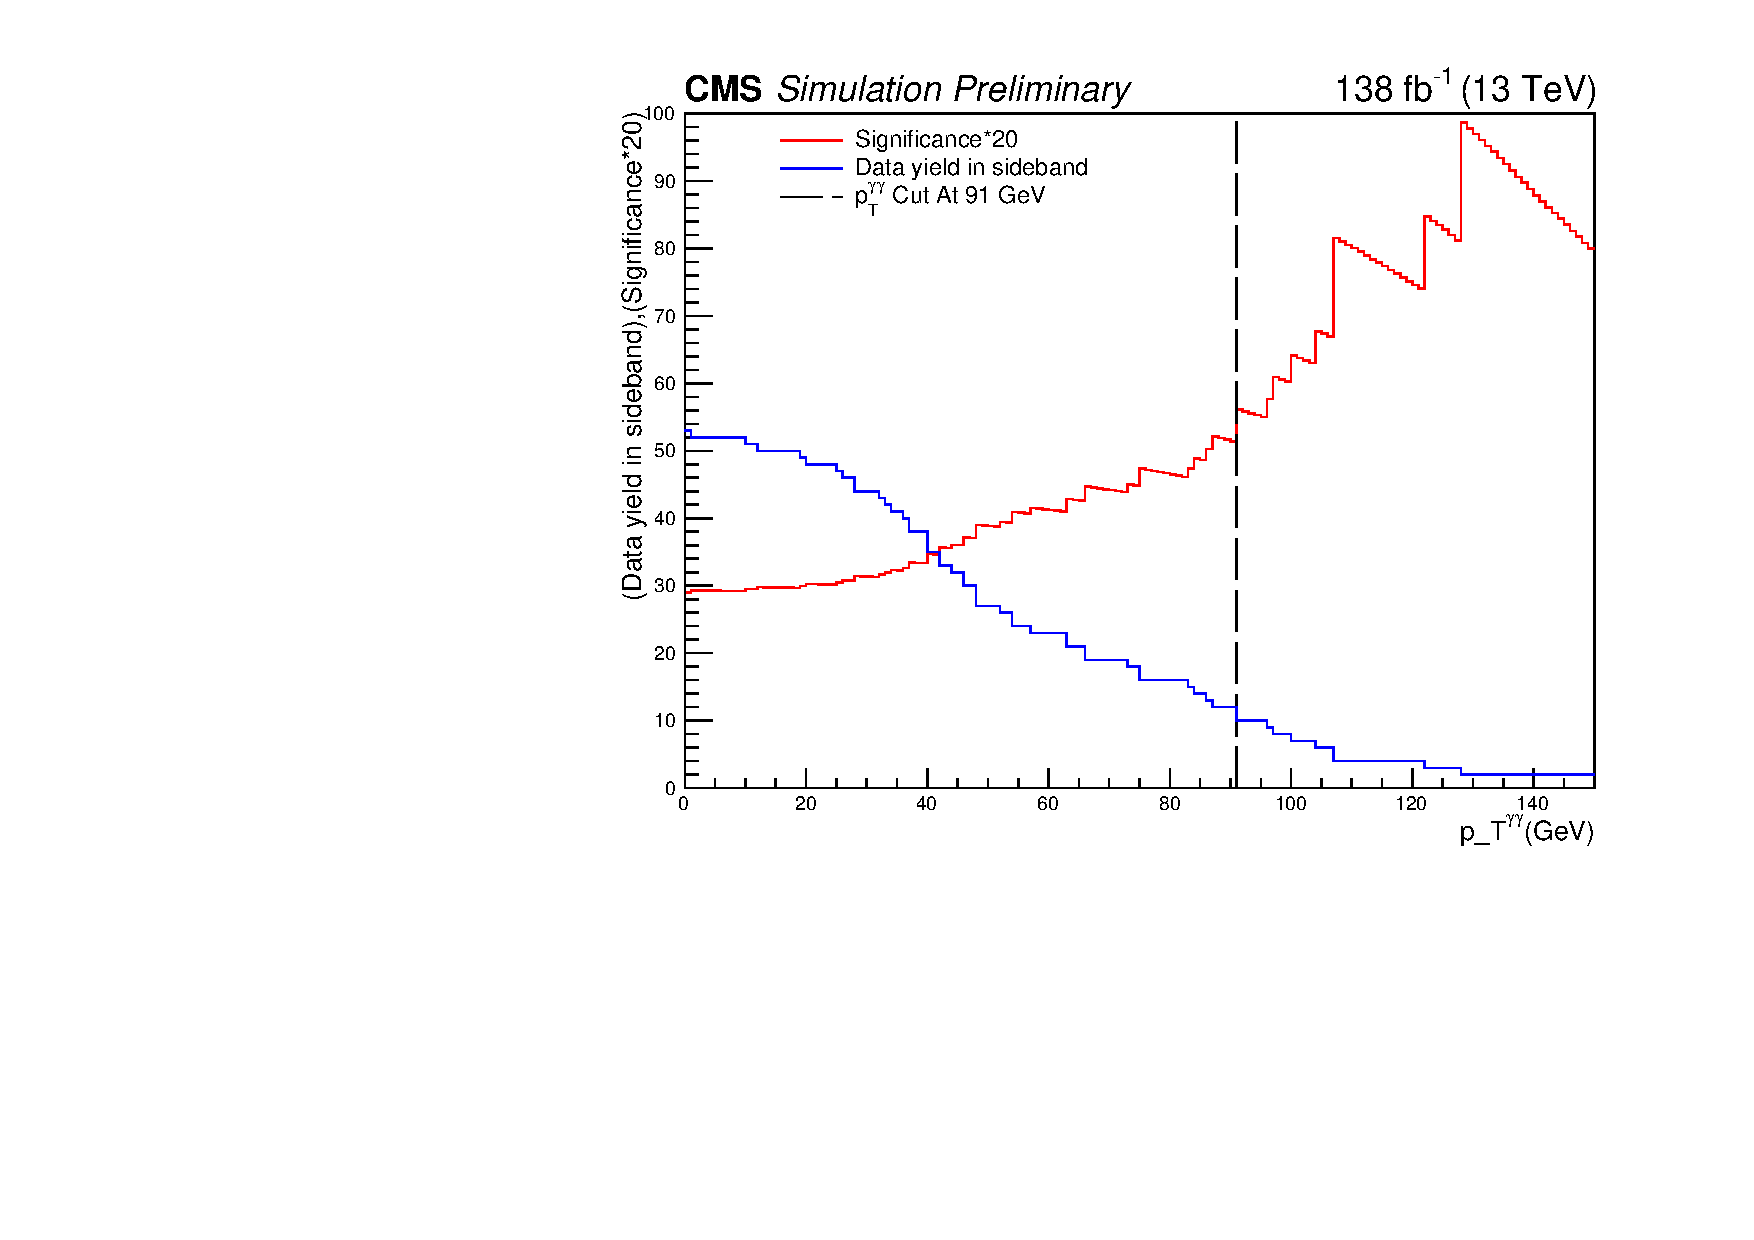
\includegraphics[width=0.47\textwidth]{Sections/HHWWgg/images/Selections/FL_CutBased/dipho_pt.pdf}}
    \subfigure{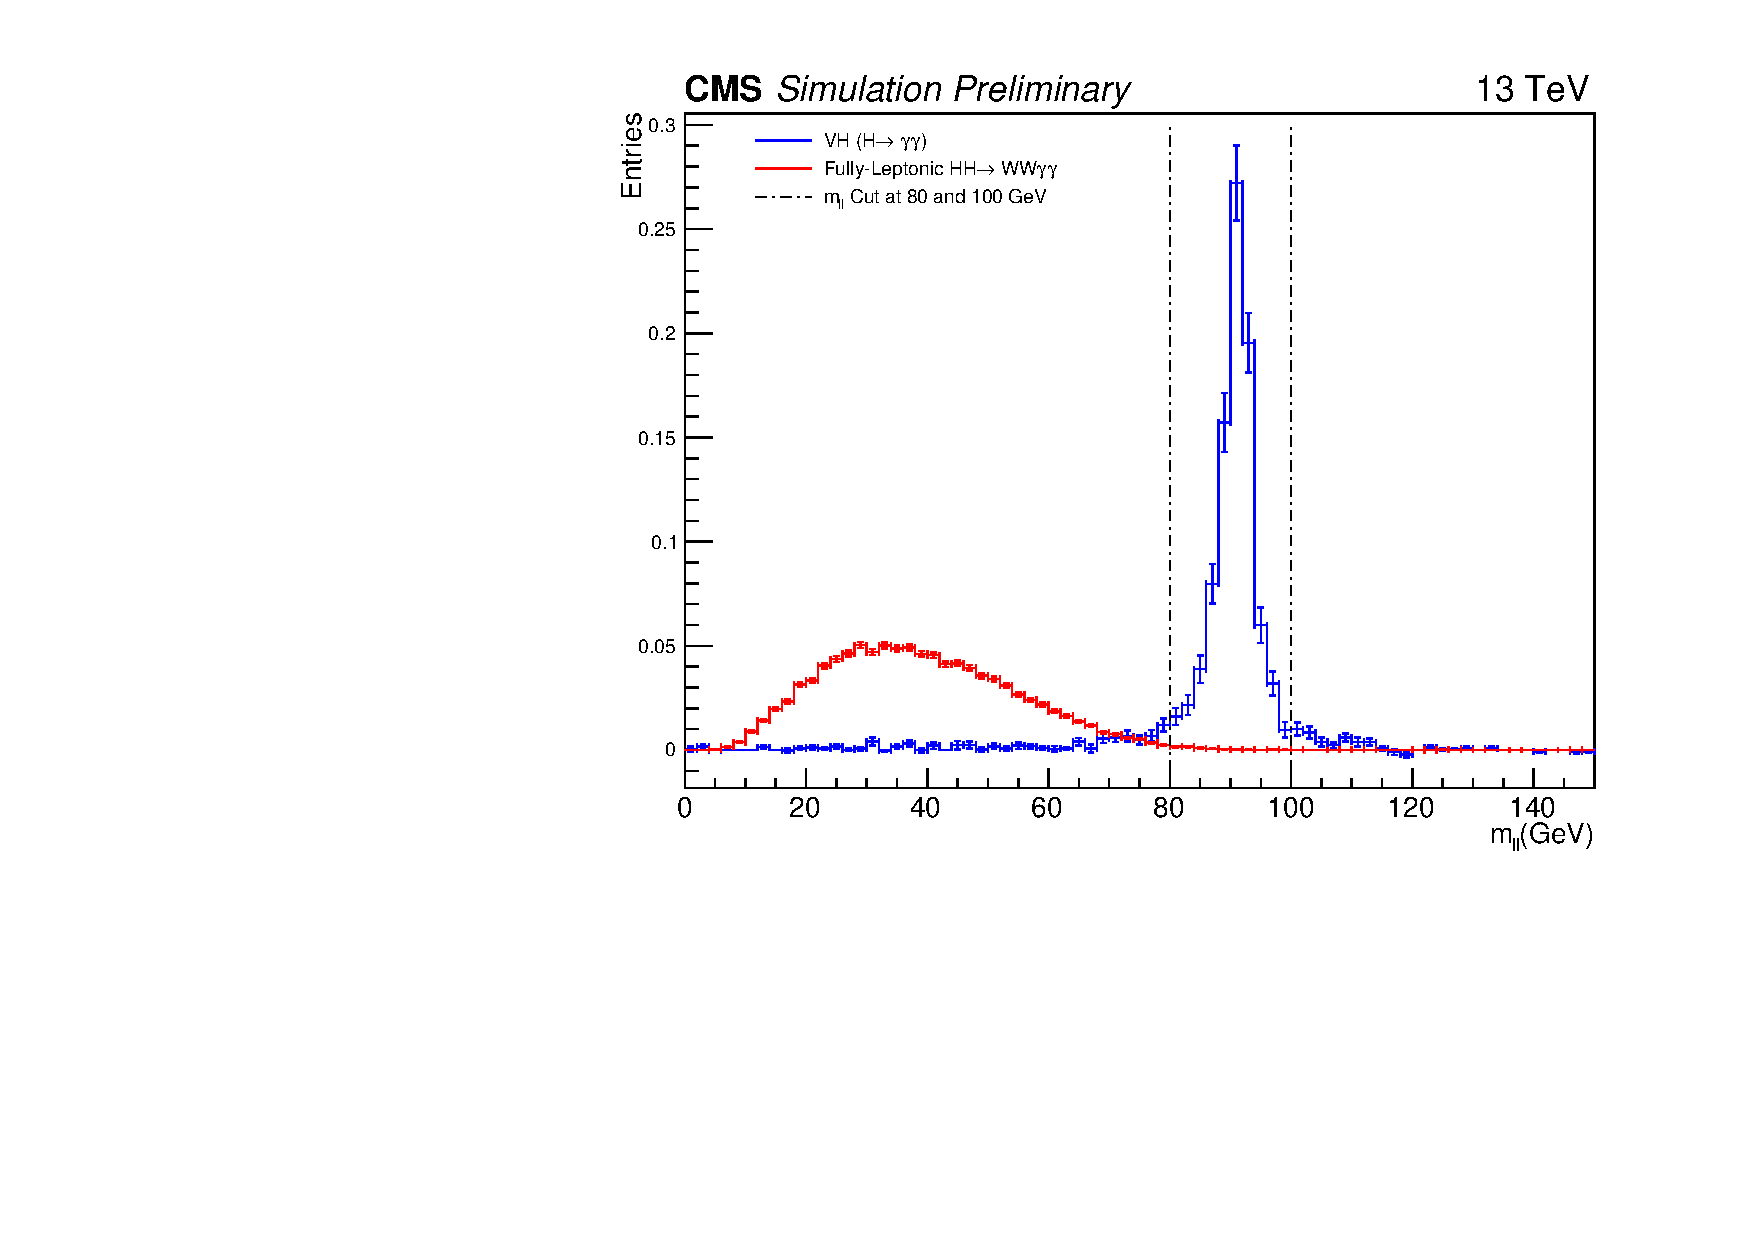
\includegraphics[width=0.47\textwidth]{Sections/HHWWgg/images/Selections/FL_CutBased/DiLeptonMass.pdf}}
    \caption{
      For fully leptonic channel: (a) Significance scan of di-photon $p_{T}$ cut, the black dashed line is the final cut value:$p_{T}$ $> 91$ GeV . (b) $m_{ll}$ distribution comparison between signal and VH events, the signal and VH have been normalized to 1, and the two dashed lines are the final cuts at di-Lepton mass: $m_{ll}$ $< 80$GeV or $m_{ll}$ $> 100$ GeV .
    }
    \label{fig:FL_support}
  \end{center}
\end{figure}

